\newpage
\section{神经网络}
%摸了
\subsection{神经元模型}

\begin{definition}
    \hl{神经网络}是由具有适应性的\hl{简单单元}组成的广泛\hl{并行互联}的网络, 它的组织能够模拟\hl{生物神经系统}对真实世界物体所作出的反应. 
\end{definition}


\begin{figure}[!htb]
    \centering
    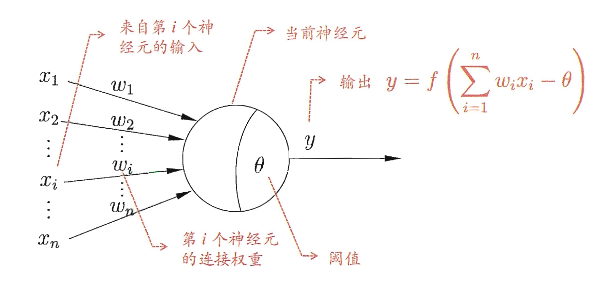
\includegraphics[width=0.42\textwidth]{pic/ML5/M-P 神经元模型}
    \caption{M-P 神经元模型}
\end{figure}
输入->处理->激活函数->输出


\begin{figure}[!htb]
    \centering
    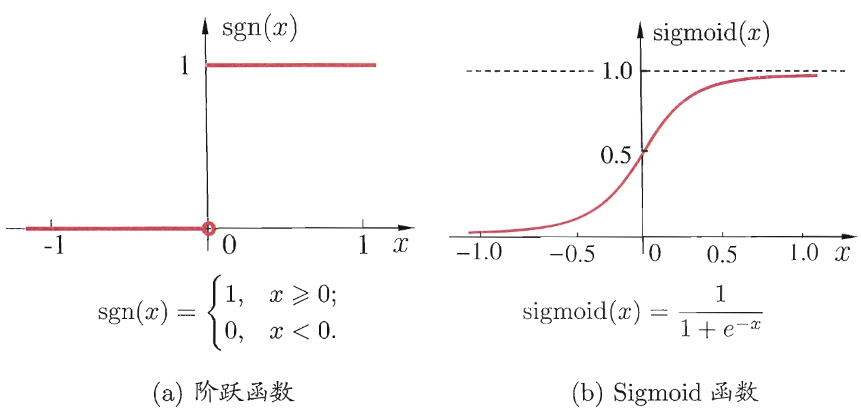
\includegraphics[width=0.42\textwidth]{pic/ML5/典型的神经元激活函数}
    \caption{典型的神经元激活函数}
\end{figure}

\subsection{感知机与多层网络}
\subsubsection{感知机}
感 知 机 (Perceptron)由 两 层 神 经 元 组 成, 输入层接收外界 输 入 信 号 后 传 递 给 输 出 层 ,输 出 层 是 M-P 神 经 元. 感知机能容易地实现逻辑与、或、非运算. 

给 定 训 练 数 据 集 , 权 重 $w_i(i=1,2,\dots,n)$ 以 及 阈 值 $\theta$ 可 通 过 学 习 得 到 . 

\begin{figure}[!htb]
    \centering
    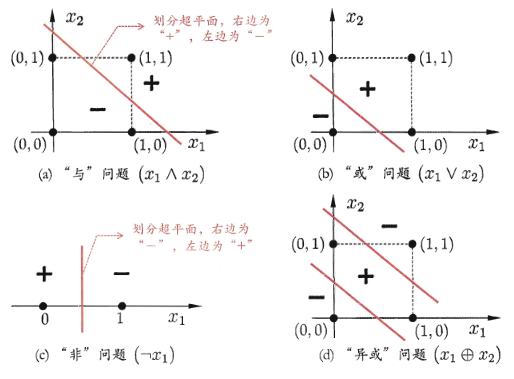
\includegraphics[width=0.42\textwidth]{pic/ML5/线 性 可 分 的 “与 “或” “非” 问 题 与 非 线 性 可 分 的 “异或” 问题}
    \caption{线 性 可 分 的 “与 “或” “非” 问 题 与 非 线 性 可 分 的 “异或” 问题}
\end{figure}

两 类 模 式 是 线 性 可 分 的 ,则 感 知 机 的 学 习 过 程 一 定 会 收 敛,  否则 感 知 机 学 习 过 程 将 会 发 生 振 荡. 单层感知机的学习能力非常有限, 只能解决线性可分问题.

\subsubsection{多层感知机}
输出层与输入层之间的一层神经元, 被称之为隐层或隐含层, 隐含层和输出层神经元都是具有激活函数的功能神经元. 

\subsubsection{多层前馈神经网络}
定义:每层神经元与下一层神经元全互联, 神经元之间不存在同层连接也不存在跨层连接.

前馈:输入层接受外界输入, 隐含层与输出层神经元对信号进行加工, 最终结果由输出层神经元输出

学习:根据训练数据来调整神经元之间的“连接权”以及每个功能神经元的“阈值”

\subsection{误差逆传播算法}
误差逆传播(Error BackPropagation,简 称 BP ) 算法是迄今最成功的神经网络学习算法. 

给 定 训 练 集 $D=\{ (\bx_1, \by_1), (\bx_2,\by_2),\dots,(\bx_m,\by_m) \}$, $\bx_i\in\R^d$, $\by_i\in\R^l$, 即输入示例由 $d$ 个属性描述, 输出 $l$ 维实值向量. 以拥有 $d$ 个输入神经元、,$l$ 个输出神经元、$q$ 个隐层神经元的多层前馈网络结构为例

\begin{figure}[!htb]
    \centering
    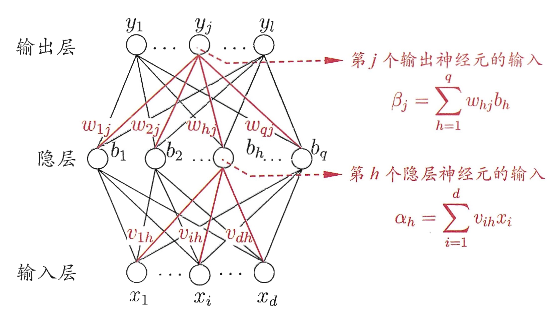
\includegraphics[width=0.42\textwidth]{pic/ML5/B P 网络及算法中的变量符号}
    \caption{BP 网络及算法中的变量符号}
\end{figure}

\begin{itemize}
    \item $\theta_j$: 输出层第 $j$ 个神经元阈值
    \item $\gamma_h$: 隐含层第 $h$ 个神经元阈值
    \item $v_{ih}$: 输入层与隐层神经元之间的连接权重
    \item $w_{hj}$: 隐层与输出层神经元之间的连接权重
\end{itemize}

BP 算法基于梯度下降(gradient descent)策略,以目标的负梯度方向对参数进行调整. 误差 $E_k$ 给定学习率 $\eta$ 
\begin{align*}
    \Delta w_{hj}=-\eta\pard{E_k}{w_{hj}}
\end{align*}

标准BP 与 累计 BP

多层前馈网络表示能力: 只需一个包含足够多神经元的隐层,多层前馈网络就能以任意精度逼近任意复杂度的连续函数. 

缓解过拟合的策略:
\begin{itemize}
    \item 早停
    \item 正则化 (惩罚复杂性)
\end{itemize}

\subsection{全局最小与局部最小}
定义了全局最小与局部最小

以及跳出局部最小的方法

\subsection{其他常见神经网络}
\begin{itemize}
    \item RBF
    \item ART
    \item SOM
    \item 级联相关
    \item Elman
    \item Boltzmann
\end{itemize}
\subsection{深度学习}
典型的深度学习模型就是很深层的神经网络